\documentclass[a4paper]{report}
\usepackage[utf8]{inputenc}
\usepackage[portuguese]{babel}
\usepackage{hyperref}
\usepackage{a4wide}
\hypersetup{pdftitle={Trabalho 1},
pdfauthor={João Teixeira, José Ferreira, Miguel Solino},
colorlinks=true,
urlcolor=blue,
linkcolor=black}
\usepackage{subcaption}
\usepackage[cache=false]{minted}
\usepackage{listings}
\usepackage{booktabs}
\usepackage{multirow}
\usepackage{appendix}
\usepackage{tikz}
\usepackage{authblk}
\usepackage{bashful}
\usepackage{verbatim}
\usetikzlibrary{positioning,automata,decorations.markings}

\begin{document}

\title{Trabalho 1\\ 
\large Grupo Nº 3}
\author{João Teixeira (A85504) \and José Ferreira (A83683) \and Miguel Solino (A86435)}
\date{\today}

\begin{center}
    \begin{minipage}{0.75\linewidth}
        \centering
        
\includegraphics[width=0.4\textwidth]{images/eng.jpeg}\par\vspace{1cm}
        \vspace{1.5cm}
        \href{https://www.uminho.pt/PT}
        {\color{black}{\scshape\LARGE Universidade do Minho}} \par
        \vspace{1cm}
        \href{https://www.di.uminho.pt/}
        {\color{black}{\scshape\Large Departamento de Informática}} \par
        \vspace{1.5cm}
        \maketitle
    \end{minipage}
\end{center}

\tableofcontents

\pagebreak

\chapter{Introdução}

\chapter{Problema}
Observando os números de inscrição dos membros do grupo, constatamos
que o maior pertencia ao aluno Miguel Solino (86435).
Fazendo \textit{pattern matching} para o padrão ABCDE e seguindo as
regras definidas no enunciado, concluímos que a orientação das ruas é:

\begin{enumerate}
    \item A é igual a 8;
    \item B é igual a 6, logo é par, e por isso aponta para baixo;
    \item C é igual a 4, logo é par, e por isso aponta para a direita;
    \item D é igual a 3, logo é ímpar, e por isso aponta para cima;
    \item E é igual a 5, logo é ímpar, e por isso aponta para a esquerda;
\end{enumerate}

Assim, conclui-se que o problema a resolver é representado pela seguinte
imagem:

\begin{figure}[H]
    \begin{center}
        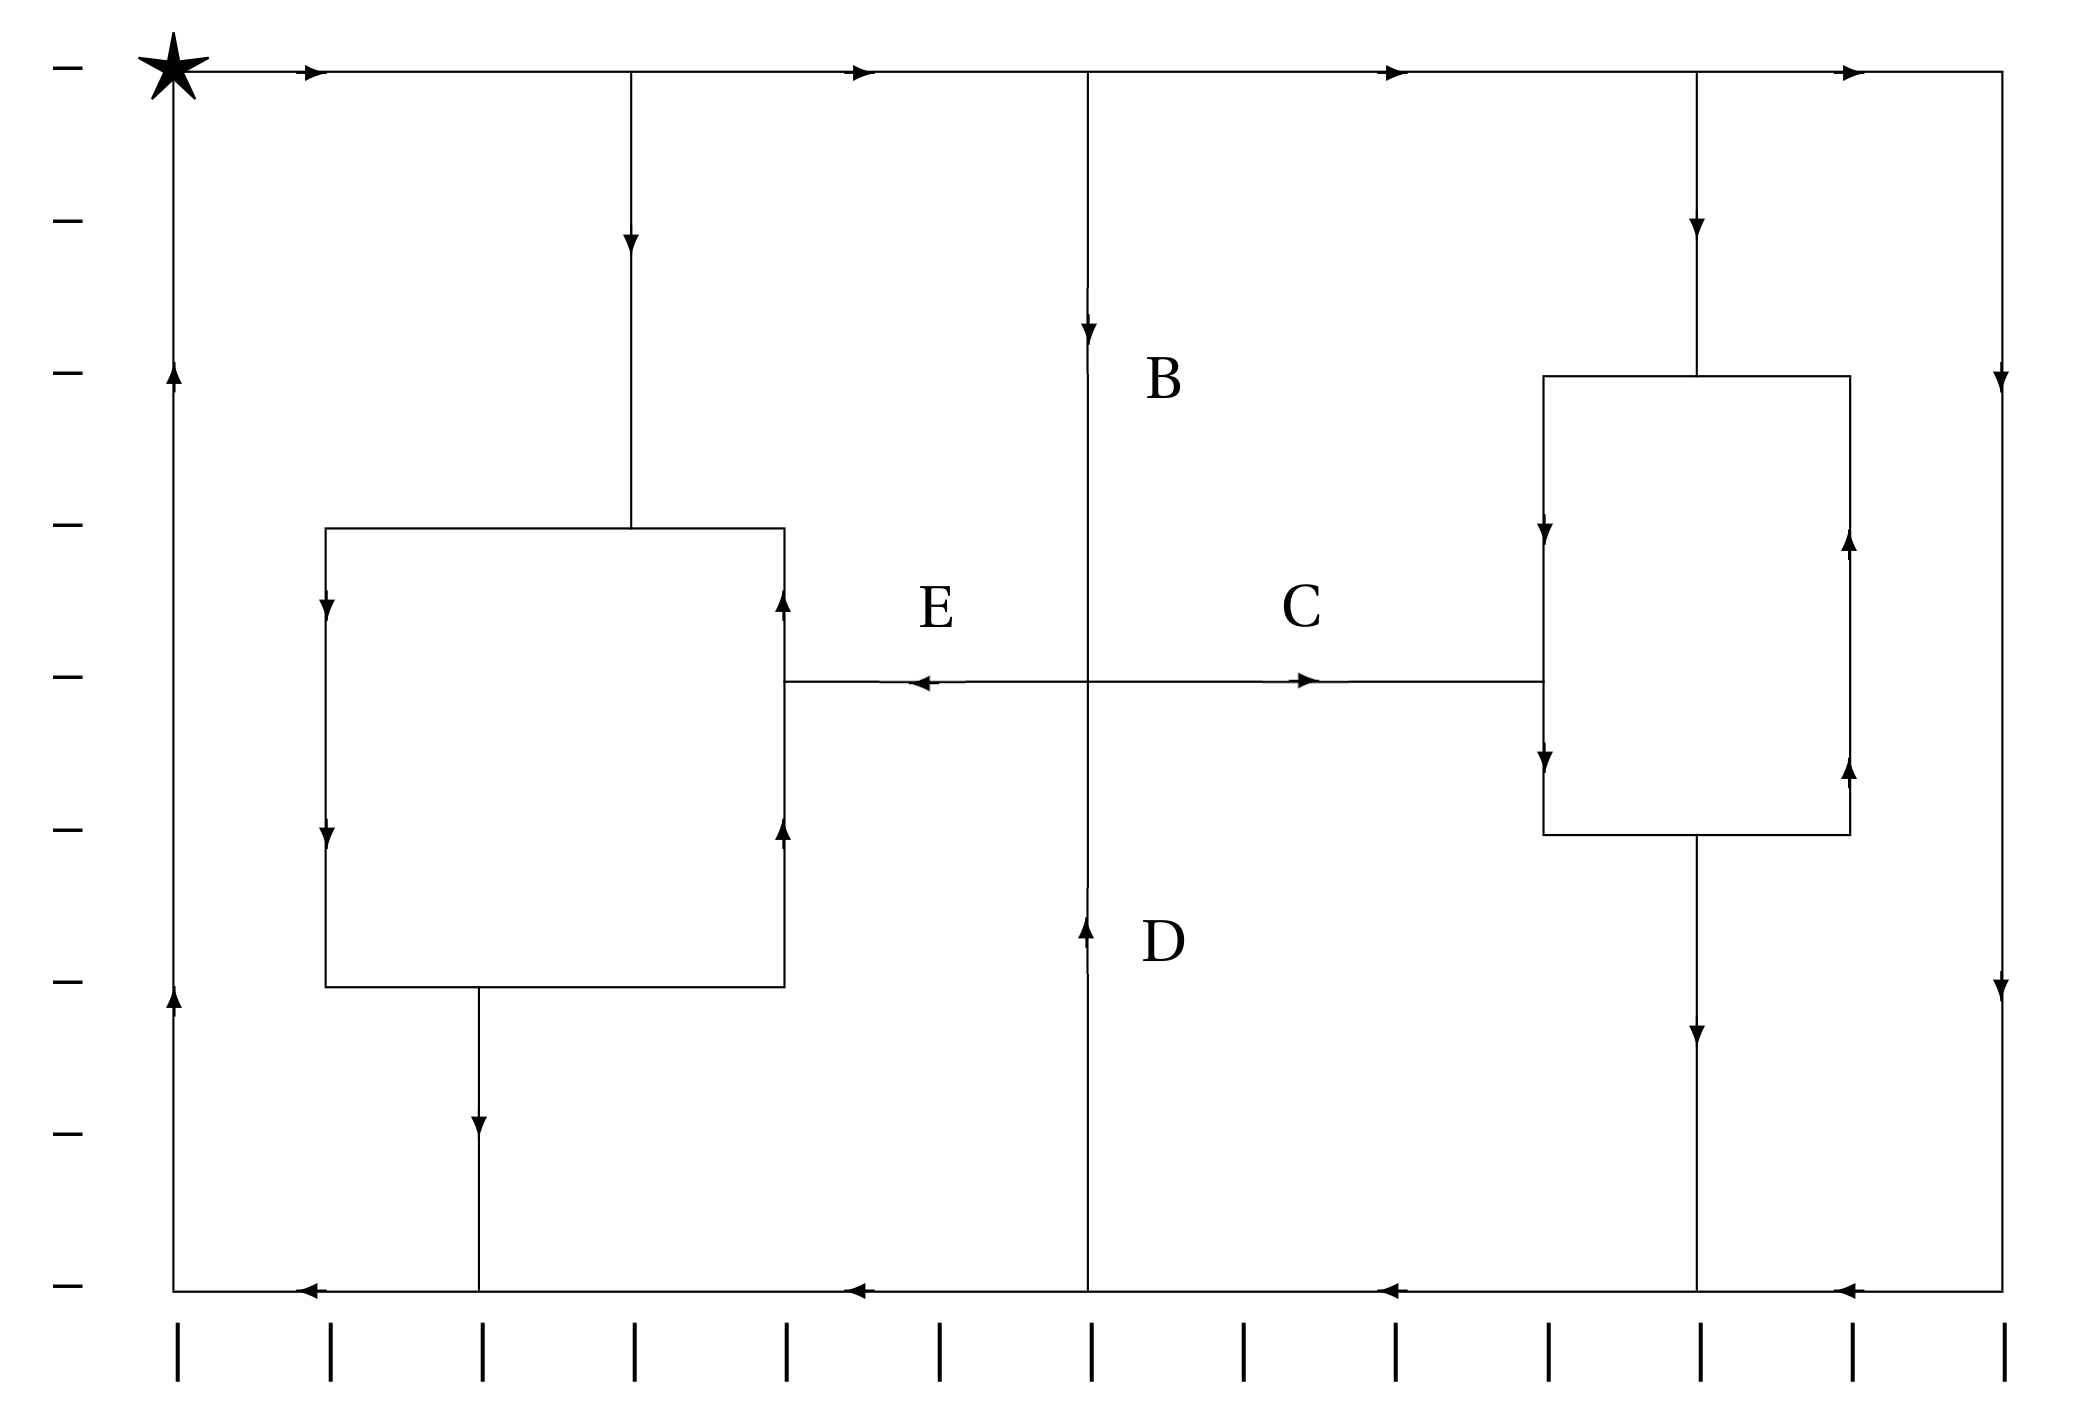
\includegraphics[width=0.8\textwidth]{images/desafio.png}\par
        \caption{representação do problema}
        \label{fig:problem}
    \end{center}
\end{figure}

\chapter{Texto de input}
\verbatiminput{../solution.lp}

\chapter{Ficheiro de output}
\bash[stdout]
lp_solve ../solution.lp
\END

\chapter{Conclusão}

\end{document}
